\chapter{Résolution des équations différentielles ordinaires}\label{Ch-ED} 

\begin{abstract}
La résolution exacte des équation différentielle fait partie des choses qui ont été demandées comme complément. Elles ne correspondent pas vraiment au but de ce document. Toutefois, le paragraphe sur la résolution numérique des équation différentielle nous a permis d'introduire des méthodes qui sont employées également dans la méthode des éléments finis (notamment la méthode de Newmark).\index[aut]{Newmark (Nathan Mortimore), 1910-1981, Américain} 
\end{abstract} 

\section{Résolution exacte des équations différentielles linéaires} 

Une \textcolorblue{Équation différentielle linéaire} est de la forme suivante:
\begin{equation}
a_0(x) y + a_1(x) y' + a_2(x) y'' + \ldots + a_n(x) y^{(n)}= f(x)
\end{equation}
où les coefficients~$a_i(x)$ sont des fonctions numériques continues. Si les fonctions~$y$ dépendent d'une seule variable~$x$, alors ces équation différentielle sont dites équation différentielle linéaires scalaires, si c'est un vecteur elles sont dites équation différentielle linéaires vectorielles ou système différentiel linéaire. Dans ce dernier cas, les~$a_i$ sont des applications linéaires. L'\textcolorblue{ordre} d'une équation différentielle est le degré non nul le plus des~$a_i$, ici~$n$. 
La méthode générale consiste à résoudre d'abord l'\textcolorblue{équation homogène}, i.e. sans second membre, i.e.~$f(x)=0$, qui donne une solution contenant une ou des «constantes d'intégration» que l'on identifie ensuite en appliquant la forme générale trouvée à l'équation avec second membre. 
 
\medskip
\subsection{Équation différentielle linéaire scalaire d'ordre 1} 

Il s'agit du cas particulier:
\begin{equation}
a(x)y' + b(x)y = c(x)
\end{equation}
où~$a$, $b$ et~$c$ sont des fonctions (connues). 

\medskip
\subsubsection{Coefficients constants} 

Si~$a$ et~$b$ sont des constantes, alors l'équation homogène précédente s'écrit sous la forme:
\begin{equation}
y' = ky
\end{equation}
avec~$k\in\RR$, et la solution est:
\begin{equation}
f(x) = C\mathrm{e}^{kx}
\end{equation}
où la constante~$C\in\RR$ est déterminée à l'aide des conditions initiales:
\begin{itemize}
\item si pour~$x_0$ on a~$f(x_0) = y_0$ alors~$C = y_0\mathrm{e}^{-kx_0}$. 
\item si~$c=0$, alors la solution du problème est celle de l'équation homogène et on a fini le travail.
\end{itemize} 
Ce type d'équation se retrouve: 
\begin{itemize} 
\item~$k<0$: modélisation de la décroissance radioactive dans un milieu homogène et fermé; 
\item~$k>0$: modélisation de la croissance d'une population (modèle simplifié car en milieu fermé, cette croissance ne peut durer indéfiniment). 
\end{itemize} 
Si~$c\ne0$, il faut déterminer une solution particulière de l'équation avec second membre. On appliquera les mêmes techniques que dans le cas des coefficients non constants (voir ci-après). 

\medskip
\subsubsection{Coefficients non constants} 

\paragraph{1. Traitement de l'équation homogène}

On réécrit l'équation homogène:
\begin{equation}
y' + \frac{b(x)}{a(x)} y = 0
\end{equation}
sur un intervalle~$I$ où~$a(x)$ ne s'annule pas. Ensuite, en notant~$A(x)$, une primitive de la fonction~$b(x)/a(x)$, il vient:
\begin{equation}
y' + A'(x) y =0
\end{equation}
puis:
\begin{equation}
y' \mathrm{e}^{A(x)} + y \frac{b(x)}{a(x)} \mathrm{e}^{A(x)} =0
\end{equation}
et:
\begin{equation}
y' \mathrm{e}^{A(x)} + y A'(x) \mathrm{e}^{A(x)}=0
\end{equation}
qui est de la forme~$u' v + u v'$ et vaut~$ (u v)'$, d'où:
\begin{equation}
\frac{\mathrm d}{\d x}(y \mathrm{e}^{A(x)})=0
\end{equation}
soit:
\begin{equation}
y \mathrm{e}^{A(x)} = C
\end{equation}
Les solutions sont alors les fonctions, définies sur~$I$, de la forme:
\begin{equation}\label{eq:ed:forme}
y(x) = C \mathrm{e}^{-A(x)}
\end{equation}
où encore une fois la constante~$C\in\RR$ est déterminée par les conditions initiales. 

\medskip
\paragraph{2. Solution particulière}

Plusieurs cas se présentent:
\begin{itemize}
\item~$c(x)=0$: la solution du problème est celle de l'équation homogène et on a fini;
\item~$c(x)\ne0$: il faut déterminer une solution particulière de l'équation avec second membre. Cela n'est pas toujours simple car la forme de cette solution particulière varie en fonction de~$c(x)$;
\item~$c(x)=\text{C\fup{te}}$: la quantité~$f_0=c/b$ est aussi une constante et l'ensemble des solutions est donc~$f=y(x)+f_0$;
\item~$c(x)$ est une somme de fonctions:~$f_0$ est alors la somme des solutions particulières obtenues pour chacun des termes de la somme constituant~$c(x)$;
\item~$c(x)$ est un polynôme de degré~$n$:~$f_0$ est également un polynôme de degré~$n$;
\item~$c(x) = A\cos(\omega x + \varphi) + B \sin(\omega x + \varphi)$: on cherche~$f_0$ comme combinaison linéaire de~$\cos(\omega x + \varphi)$ et~$\sin(\omega x + \varphi)$, i.e. sous la même forme que~$c(x)$. 
\end{itemize}
Dans le cas général, on utilise la méthode dite de la \textcolorblue{variation des constantes} qui consiste à se ramener, par un changement de fonction variable, à un problème de calcul de primitive. On suppose que, sur l'intervalle d'étude, la fonction~$a(x)$ ne s'annule pas\footnote{Il est possible de résoudre sur plusieurs intervalles de type~$I$ et essayer de «recoller» les solutions.}. On connait déjà la solution générale~\eqref{eq:ed:forme} de l'équation homogène. On décide d'étudier le cas de la fonction~$z(x)$ définie par:
\begin{equation}
z(x) = k(x)\mathrm{e}^{- A(x)}
\end{equation}
en substituant dans~$y(x)$ la fonction~$k(x)$ à la constante~$C$, d'où le nom de la méthode. En reportant dans l'équation différentielle initiale, il vient:
\begin{equation}
a(x)k'(x) = c(x)\mathrm{e}^{A(x)}
\end{equation}
qui est une équation différentielle dépendant cette fois de la fonction~$k(x)$. Si on note~$B(x)$ une primitive de la fonction~$c(x) \mathrm{e}^{A(x)}/a(x)$, l'ensemble des solutions est alors:
\begin{equation}
k(x) = B(x) + C
\end{equation}
et la solution générale s'écrit alors sous la forme:
\begin{equation}
f(x) = (B(x) + C) \mathrm{e}^{-A(x)}
\end{equation}
soit, finalement:
\begin{equation}
f = \exp\left( -\int\frac{b(x)}{a(x)}\d x \right) \left\{ C + \int \frac{c(x)}{a(x)} \exp\left(\int \frac{b(x)}{a(x)}\d x \right)\d x \right\}
\end{equation}
On peut évidemment être confronté à un calcul d'intégral qui n'est pas simple (ou même pas possible à l'aide des fonctions usuelles). 
 
\medskip
\subsection{Équation différentielle du premier ordre à variables séparées} 

Une \textcolorblue{équation différentielle d'ordre un à variables séparées} est une équation différentielle qui peut se mettre sous la forme:
\begin{equation}
y' = f(x)g(y)
\end{equation}
Dans un tel problème, on commence par chercher les \textcolorblue{solutions régulières} qui sont les solutions telles que~$g(y)$ n'est jamais nul. Comme~$g(y)\ne0$, on peut écrire l'équation sous la forme:
\begin{equation}
\frac{1}{g(y(x))} y'(x) = f(x)
\end{equation}
par rapport à la variable~$x$, ce qui conduit à:
\begin{equation}
\int_{x_0}^x \frac{1}{g(y(u))}y'(u) \d u = \int_{x_0}^x f(u) \d u 
\end{equation}
et qui après changement de variable, est de la forme:
\begin{equation}
\int_{y_0}^y \frac{1}{g(v)} \d v = \int_{x_0}^x f(u) \d u 
\end{equation}
L'hypothèse~$g(y)\ne0$ écarte certaines solutions particulières. Par exemple, si~$y_0$ est un point d'annulation de~$g$, alors la fonction constante égale à~$y_0$ est une solution maximale de l'équation. Une telle solution, dite \textcolorblue{solution singulière}, est donc telle que~$g(y)$ est toujours nul. Si la seule hypothèse faite sur~$g$ est la continuité, il peut exister des solutions «hybrides» constituées du raccordement de solutions régulières et singulières. D'une manière générale, pour une solution donnée, la quantité~$g(y)$ sera soit toujours nulle, soit jamais nulle. 

Il existe un cas particulier, qui est celui de \textcolorred{l'équation différentielle d'ordre un à variables séparées autonome} qui s'écrit:
\begin{equation}
y' = g(y)
\end{equation}
c'est-à-dire que la relation formelle ne dépend pas de~$x$. Dans ce cas, si~$x \mapsto y_0(x)$ est une solution, les fonctions obtenues par translation de la variable, de la forme~$x \mapsto y_0(x+A)$, sont également solutions. Il y a en outre une propriété de monotonie, au moins pour les solutions régulières: puisque~$g$ ne s'annule pas, il garde alors un signe constant. 
 
\medskip
\subsection{Équation différentielle linéaire d'ordre deux} 

Les équations différentielles linéaires d'ordre deux sont de la forme:
\begin{equation}
a(x)y'' + b(x)y' + c(x)y = d(x)
\end{equation}
où~$a(x)$, $b(x)$, $c(x)$ et~$d(x)$ sont des fonctions. Si elles ne peuvent pas toutes être résolues explicitement, beaucoup de méthodes existent. 

\medskip
\subsubsection{Équation différentielle homogène} 

Pour l'équation différentielle homogène ($d(x)=0$), une somme de deux solutions est encore solution, ainsi que le produit d'une solution par une constante. L'ensemble des solutions est donc un espace vectoriel et contient notamment une solution évidente, la fonction nulle. 

\medskip
\subsubsection{Équation différentielle homogène à coefficients constants} 

On cherche des solutions sous forme exponentielle~$f(x) = \mathrm{e}^{\lambda x}$. Une telle fonction sera solution de l'équation différentielle si et seulement si$\lambda$ est solution de l'\textcolorblue{équation caractéristique} de l'équation différentielle:
\begin{equation}
a\lambda^2 + b\lambda + c = 0
\end{equation}
Comme pour toute équation du second degré, il y a trois cas correspondant au signe du discriminant~$\Delta$:
\begin{enumerate}
\item$\Delta>0$ --- L'équation caractéristique possède deux solutions~$\lambda_1$ et~$\lambda_2$, et les solutions de l'équation différentielle sont \textcolorred{engendrées} par~$f_1(x) = \mathrm{e}^{\lambda_1x}$ et~$f_2(x) = \mathrm{e}^{\lambda_2x}$, i.e. de la forme:
\begin{equation}
f(x) = C_1f_1(x) + C_2f_2(x)
\end{equation}
les constantes réeles~$C_1$ et~$C_2$ étant définies par: 
\begin{itemize} 
\item les conditions initiales: en un point (instant) donné~$x_0$, on spécifie les valeurs de~$y_0=y(x_0)$ et~$y'_0=y'(x_0)$. Dans ce cas l'existence et l'unicité de la solution vérifiant ces conditions initiales sont garanties. 
\item les conditions aux limites: pour de nombreux problèmes physiques, il est fréquent de donner des conditions aux limites en précisant les valeurs~$y_1$et~$y_2$ aux instants~$x_1$ et~$x_2$. Il y a alors fréquemment existence et unicité des solutions, mais ce n'est pas toujours vrai. 
\end{itemize} 
\item$\Delta=0$ --- L'équation caractéristique possède une solution double~$\lambda$, et les solutions de l'équation différentielle sont de la forme:
\begin{equation}
f(x) = (C_1 x + C_2)\mathrm{e}^{\lambda x}
\end{equation}
les constantes réelles~$C_1$ et~$C_2$ étant définies comme précédemment. 
\item$\Delta<0$ --- L'équation caractéristique possède deux solutions~$\lambda_1$ et~$\lambda_2$ complexes conjuguées, et les solutions de~$\RR$ dans~$\CC$ de l'équation différentielle sont \textcolorred{engendrées} par~$f_1(x) = \mathrm{e}^{\lambda_1x}$ et~$f_2(x) = \mathrm{e}^{\lambda_2x}$, i.e. de la forme:
\begin{equation}
f(x) = C_1f_1(x) + C_2f_2(x)
\end{equation}
où cette fois~$C_1$ et~$C_2$ sont des complexes. Comme on cherche des solutions de~$\RR$ dans~$\RR$, on note~$\lambda_1 = u + iv$ (et donc~$\lambda_2 = u -iv$), on exprime~$f_1$ et~$f_2$, et on déduit que les fonctions~$g_1$ et~$g_2$, à valeurs dans~$\RR$ cette fois, sont encore solutions:
\begin{align}
&g_1(x) =\frac 12 (f_1(x) + f_2(x) )= \mathrm{e}^{ux}\cos(vx)\\
&g_2(x) = \frac{1}{2i}(f_1(x) - f_2(x)) = \mathrm{e}^{ux}\sin(vx)
\end{align}
et engendrent encore l'ensemble des solutions. On a donc les solutions sous la forme:
\begin{equation}
f(x) = \mathrm{e}^{ux}(C_1\cos(vx) + C_2\sin(vx))
\end{equation}
les constantes réelles~$C_1$ et~$C_2$ étant définies comme précédemment. Notons que~$f(x)$ s'écrit également:
\begin{equation}
f(x) = q \mathrm{e}^{ux}\cos(vx+r)
\end{equation}
avec~$q$ et~$r$ deux réels à déterminer comme précédemment. Cette forme est parfois plus pratique selon les problèmes. 
\end{enumerate}

\medskip
\subsubsection{Équation différentielle homogène à coefficients non constants}

Si les fonctions~$a(x)$, $b(x)$ et~$c(x)$ ne sont pas constantes, alors il n'existe pas d'expression générale des solutions. C'est pour cette raison qu'au \textsc{xix}\fup{e} siècle furent introduites de nombreuses fonctions spéciales, comme les fonctions de Bessel\index[aut]{Bessel (Friedrich Wilhelm), 1784-1846, Allemand} ou la fonction d'Airy,\index[aut]{Airy (George Biddell, Sir -), 1801-1892, Anglais} définies comme solutions d'équations qu'il est impossible de résoudre explicitement. 

Toutefois, dès lors qu'une solution particulière non nulle de l'équation est connue, il est possible de la résoudre complètement. En effet, le théorème de Cauchy-Lipschitz\index[aut]{Cauchy (Augustin Louis, baron -), 1789-1857, Français}\index[aut]{Lipschitz (Rudolph Otto Sigismund), 1832-1903, Allemand} affirme que l'ensemble des solutions de l'équation constitue un espace vectoriel de dimension deux. Résoudre l'équation différentielle revient donc à exhiber deux fonctions solutions non proportionnelles: elles formeront une base de l'espace des solutions. Une telle base est appelée \textcolorblue{système fondamental de solutions}. 

\medskip
\subsubsection{Solution particulière et traitement du second membre} 

On peut agir de la même manière que pour les équation différentielle d'ordre un, et les mêmes remarques s'appliquent. On résout l'équation homogène puis on cherche une solution de l'équation avec second membre pour les connaître toutes. 

Les équation différentielle d'ordre deux correspondent typiquement en physique aux problèmes dynamiques. Même si dans le cas réel on n'a rarement des phénomènes linéaires, des hypothèses de petits mouvements permettent de s'y ramener. Si cette hypothèse de petits déplacements ne peut être vérifier, on aura alors recourt à des techniques dites de linéarisation, ou à des méthodes numériques comme la méthode de Newmark\index[aut]{Newmark (Nathan Mortimore), 1910-1981, Américain} (qui sera présentée un petit peu plus loin).
 
\medskip
\section{Résolution numérique} 

\sbox{\MaBoiteAvecPhotos}{\setlength{\tabcolsep}{0pt}\scriptsize%
\begin{tabular}{cccc} 
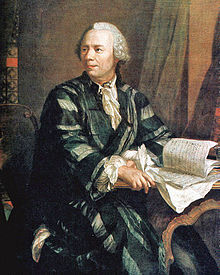
\includegraphics[height=25mm]{Euler}& 
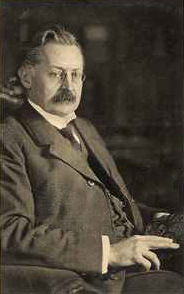
\includegraphics[height=25mm]{Runge}& 
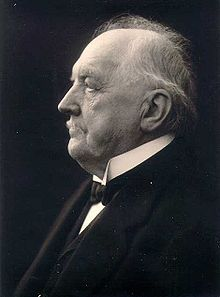
\includegraphics[height=25mm]{Kutta}& 
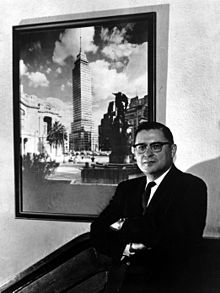
\includegraphics[height=25mm]{Newmark}\\ 
Euler & Runge& Kutta& Newmark\end{tabular}}
\medskip
\begin{histoire}
La première méthode numérique fut introduite en 1768 par Leonhard Euler.\index[aut]{Euler (Leonhard Paul), 1707-1783, Suisse}\\
\ImageAGauche{%
Depuis, un grand nombre de techniques ont été développées: elles se basent sur la discrétisation de l'intervalle d'étude en un certain nombre de pas. Suivant le type de formule utilisé pour approcher les solutions, on distingue les méthodes numériques à un pas ou à pas multiples, explicites ou implicites. \\
\indent
Il existe plusieurs critères pour mesurer la performance des méthodes numériques: la consistance d'une méthode indique que l'erreur théorique effectuée en approchant la solution tend vers zéro avec les pas. La stabilité indique la capacité à contrôler l'accumulation des erreurs d'arrondi. Ensemble elles assurent la convergence, i.e. la possibilité de faire tendre l'erreur globale vers zéro avec le pas. Ces notions seront posées brièvement
au chapitre~\ref{Ch-shemanum}.}
\end{histoire}

Dans le cas d'équation différentielle non linéaires, on passera forcément à une résolution numérique. Mais les méthodes numériques permettent évidemment aussi de résoudre numériquement les équations différentielles et les équations aux dérivées partielles.

L'idée générale est toujours la même: on approche la dérivée d'une fonction en un point par sa tangente (ce qui revient finalement à la définition de la dérivée). Pour une fonction~$f(x)$, on écrit donc au point~$x=a$ une relation de la forme:
\begin{equation}
f'(a)\approx \frac{f(b)-f(c)}{b-c}
\end{equation}
où~$b$ et~$c$ sont d'autres points. Par exemple, pour~$c=a$ et~$b=a+\varepsilon$ on obtient un schéma décentré à droite; pour~$c=a-\varepsilon$ et~$b=a+\varepsilon$, on ontient un schéma centré.
 
\medskip
\subsection{Méthode d'Euler, Runge-Kutta ordre 1}\index{méthode de Runge-Kutta! ordre 1}\index{méthode d'Euler}\index[aut]{Euler (Leonhard Paul), 1707-1783, Suisse}\index[aut]{Kutta (Martin Wilhelm), 1867-1944, Allemand}\index[aut]{Runge (Carl David Tolmé), 1856-1927, Allemand} 

Soit à résoudre l'équation différentielle suivante:
\begin{equation}
y' = f(t, y), \qquad y(t_0) = y_0
\end{equation}
D'après ce qui précède, on utilise une discrétisation de pas~$h$, ce qui donne comme point courant~$y_i=y_0+ih$, et on fait l'approximation:
\begin{equation} 
y'=\frac{y_{i+1}-y_i}h
\end{equation}
On obtient alors le schéma numérique:
\begin{equation}
y_{i+1}=y_i+hf(t,y_i)
\end{equation}
qui permet d'obtenir~$y_{i+1}$ uniquement en fonction de données au pas~$i$. Cette méthode due à Euler, correspond également à la méthode de Runge-Kutta à l'ordre 1.\index{méthode de Runge-Kutta! ordre 1}\index{méthode d'Euler}\index[aut]{Euler (Leonhard Paul), 1707-1783, Suisse}\index[aut]{Kutta (Martin Wilhelm), 1867-1944, Allemand}\index[aut]{Runge (Carl David Tolmé), 1856-1927, Allemand} 
 
\medskip
\subsection{Méthode de Runge-Kutta d'ordre 2}\index{méthode de Runge-Kutta! ordre 2}\index[aut]{Kutta (Martin Wilhelm), 1867-1944, Allemand}\index[aut]{Runge (Carl David Tolmé), 1856-1927, Allemand} 

La méthode de Runge-Kutta à l'ordre 2 est obtenue par amélioration de la méthode d'Euler en considérant le point milieu du pas~$h$. Ainsi, on écrit cette fois:
\begin{equation}
y_{i+1}=y_i+h.f\left(t+\frac{h}2,y_i+\frac{h}2f(y,y_i)\right)
\end{equation}
Mézalor me direz-vous, il manque des bouts... Les dérivées au milieu du pas d'intégration sont obtenues par:
\begin{equation}
y_{i+\frac{1}{2}} = y_i + \frac{h}{2} f \left( t, y_i \right) \qquad \text{ et } \qquad y'_{i+\frac{1}{2}} = f \left( t + \frac{h}{2}, y_{i+\frac{1}{2}} \right)
\end{equation}
En réinjectant cela, on obtient sur le pas~$h$ complet:
\begin{equation}
y_{i+1} = y_i + h y'_{i+\frac{1}{2}}
\end{equation}
Notons qu'il s'agit du cas centré ($\alpha=1/2$) de la formule plus générale:
\begin{equation}
y_{i+1} = y_i + h\left[\left(1-\frac1{2\alpha}\right)f \left( t, y_i \right) + \frac1{2\alpha}f \left( t + \alpha\,h, y_i + \alpha\,h f \left( t, y_i \right) \right)\right]
\end{equation}
C'est une méthode d'ordre 2 car l'erreur est de l'ordre de~$h^3$. 

\medskip
\subsection{Méthode de Runge-Kutta d'ordre 4}\index{méthode de Runge-Kutta! ordre 4}\index[aut]{Kutta (Martin Wilhelm), 1867-1944, Allemand}\index[aut]{Runge (Carl David Tolmé), 1856-1927, Allemand} 

Aujourd'hui, le cas le plus fréquent est celui de l'ordre 4. L'idée est toujours d'estimer la pente de~$y$, mais de façon plus précise. Pour cela, on ne prend plus la pente en un point (début ou milieu), mais on utilise la moyenne pondérée des pentes obtenues en 4 points du pas. 
\begin{itemize} 
\item~$k_1 = f \left( t_i, y_i \right)~$ est la pente au début de l'intervalle; 
\item~$k_2 = f \left( t_i + {h \over 2}, y_i + {h\over 2} k_1 \right)$ est la pente au milieu de l'intervalle, en utilisant la pente~$k_1$ pour calculer la valeur de~$y$ au point~$t_i + h/2$ par la méthode d'Euler; 
\item~$k_3 = f \left( t_i + {h \over 2}, y_i + {h\over 2} k_2 \right)$ est de nouveau la pente au milieu de l'intervalle, mais obtenue en utilisant la pente~$k_2$ pour calculer~$y$; 
\item~$k_4 = f \left( t_i + h, y_i + h k_3\right)$ est la pente en fin d'intervalle, avec la valeur de~$y$ calculée en utilisant~$k_3$. 
\end{itemize} 
 On obtient finalement la discrétisation de Runge-Kutta à l'ordre 4:
\begin{equation}
y_{i+1} = y_i + {h \over 6} (k_1 + 2k_2 + 2k_3 + k_4)
\end{equation}
La méthode est d'ordre 4, ce qui signifie que l'erreur commise à chaque étape est de l'ordre de~$h^5$, alors que l'erreur totale accumulée est de l'ordre de~$h^4$. Notons enfin que toutes ces formulation sont encore valable pour des fonctions à valeurs vectorielles. 

\medskip
\subsection{Méthode de Crank-Nicolson}\index[aut]{Crank (John), 1916-2006, Américain}\index[aut]{Nicolson (Phyllis), 1917-1968, Anglaise}

La \textcolorblue{méthode de Crank-Nicolson}\index[aut]{Crank (John), 1916-2006, Américain}\index[aut]{Nicolson (Phyllis), 1917-1968, Anglaise} est un algorithme simple permettant de résoudre des systèmes d'équations différentielles partielles. 
Cette méthode utilise les différences finies en espace et la règle des trapèzes en temps pour approcher une solution du problème: 
elle est numériquement stable et quadratique pour le temps. 
On peut facilement la généraliser à des problèmes à deux ou trois dimensions.

\medskip
Si l'on considère l'équation différentielle suivante:
\begin{equation}
  \frac{\partial u}{\partial t} = F\left(u,\, x,\, t,\, \frac{\partial u}{\partial x},\, \frac{\partial^2 u}{\partial x^2}\right)
\end{equation}
alors, en notant~$u_{i}^{n}$ le terme~$u(i \Delta x,\, n \Delta t)$, le schéma est:
\begin{equation}
  \frac{u_{i}^{n + 1} - u_{i}^{n}}{\Delta t} = \frac{1}{2}\left[ F_{i}^{n + 1}\left(u,\, x,\, t,\, \frac{\partial u}{\partial x},\, \frac{\partial^2 u}{\partial x^2}\right) + F_{i}^{n}\left(u,\, x,\, t,\, \frac{\partial u}{\partial x},\, \frac{\partial^2 u}{\partial x^2}\right) \right]
\end{equation}
où la fonction~$F$ est discrétisée à l'aide des différences finies centrées en espace.

\medskip
\textcolorblue{Ce schéma est celui utilisé pour les équations paraboliques}, comme celles de mécanique des fluides.
On l'utilise également pour des problèmes de mécanique quantique, de thermodynamique hors-équilibre
et d'électromagnétisme... et pour tout phénomène pouvant être ramenés à l'étude de l'équation de la chaleur
(qui a été le cadre de son développement).

\medskip
La méthode converge en~$O(\Delta_t^2)$.
L'étude de convergence est d'ailleurs plus aisée que dans le cas des \textcolorblue{équations hyperboliques pour lesquelles la méthode de Newmark\index[aut]{Newmark (Nathan Mortimore), 1910-1981, Américain} est préférée}.

\medskip
\subsection{Méthode de Newmark}\label{Sec-Newmark}\index[aut]{Newmark (Nathan Mortimore), 1910-1981, Américain}\index{schéma!de Newmark} 

La \textcolorblue{méthode de Newmark (1959)} permet de résoudre numériquement des équation différentielle du second ordre. Elle convient, non seulement pour des systèmes différentiels linéaires, mais aussi pour des systèmes fortement non-linéaires avec une matrice de masse et une force appliquée qui peuvent dépendre à la fois de la position et du temps. Dans ce second cas, le calcul nécessite à chaque pas une boucle d'itération. 

L'idée générale reste la même: on cherche à estimer les valeurs des dérivées (premières, secondes...) à l'instant~$t$ à partir des informations disponible à l'instant précédent (au pas de temps précédent). Pour cela, on va recourir à un développement limité. Considérons l'équation de la dynamique:
\begin{equation}
M\ \ddot x(t) + C\ \dot x(t) + K\ x(t)= f(t)
\end{equation}
On fait un développement en série de Taylor:\index[aut]{Taylor (Brook), 1685-1731, Anglais} 
\begin{equation}
u_{t+\Delta_t}=u_t+\Delta_t \dot{u}_t+\frac{\Delta_t^2}2\ddot{u}_t+\beta\Delta_t^3\dddot{u} \qquad\text{ et }\qquad \dot{u}_{t+\Delta_t} = \dot{u}_t+\Delta_t\ddot{u}_t+\gamma\Delta_t^2\dddot{u}
\end{equation}
et on fait l'hypothèse de linéarité de l'accélération à l'intérieur d'un pas de temps~$\Delta_t$:
\begin{equation}
\dddot{u}=\dfrac{\ddot{u}_{t+\Delta_t}-\ddot{u}_t}{\Delta_t}
\end{equation}
Les différents \textcolorblue{schémas de Newmark} correspondent à des valeurs particulières de~$\beta$ et~$\gamma$.\index[aut]{Newmark (Nathan Mortimore), 1910-1981, Américain}\index{schéma! de Newmark} Dans le cas~$\beta=0$ et~$\gamma=1/2$, on retombe sur le schéma des \textcolorblue{différences finies centrées}.\index{schéma!des différences finies centrées} 

\textcolorgreen{La méthode de Newmark fonctionne également pour les problèmes non linéaires, mais dans ce cas la matrice de rigidité devra être réévaluée à chaque pas de temps (ainsi que celle d'amortissement dans les cas les plus compliqués).}